Chapter~\ref{chap:memo15} introduced two atomic controllers that enforced
desired safety properties when run separately. That chapter also described
how to compose components, but informally followed the convention that
components being composed do not constrain overlapping sets of
variables. However, such a restriction is natural in sampled-data systems,
for example when composing two controllers outputting to the same sets of
actuators. This raises the question: when can two such controllers be run
in parallel in order to enforce the conjunction of their respective safety
properties? More generally, when can a sampled-data system be built up
modularly from smaller components while ensuring the properties guaranteed
by each of the components and avoiding inconsistencies in the composed
system? This chapter provides a series of proof rules to address that
question.

As alluded to above, one of the challenges is in ensuring that the
specification of the discrete controller is always enabled, i.e. it always
specifies at least one successor state.  While this might seem trivial,
consider the following scenario.  Suppose we have built a module that
prevents a quadcopter from exceeding some maximum altitude.  Furthermore,
suppose we have also built another module that prevents the quadcopter from
violating some \emph{minimum} altitude.  If we have separately verified
that these two modules enforce their respective properties, we would like
to compose them in parallel to guarantee both properties simultaneously.
That is, we would like the composed system to guarantee that the system
never goes too high or too low.  However, this is not always possible; a
module could enforce the upper bound on altitude by always accelerating
downwards.  Likewise, a module could enforce the lower bound on altitude by
always accelerating upwards.  Clearly, na\"ively composing the controllers
of these modules in parallel would result in a system that gets stuck --
there is never an acceleration that both controllers can agree on.

In this chapter, we present sound techniques for resolving this and other
potential pitfalls for reusing and composing modules for sampled-data
systems.  We observed that modularity is facilitated by separating
verification into two parts: \emph{preservation} and \emph{\progress{}}.
Preservation ensures that the model guarantees the safety property
inductively, while \progress{} ensures that the system model is always
enabled.  This separation facilitates the application of several simple,
general, and powerful operators, namely substitution, conjunction, and
disjunction.  More precisely, we state sufficient conditions for applying
these operators to individual modules to produce a new sampled-data system
with the desired properties (e.g. the conjunction of the safety properties
of conjoined modules).  Crucially, these sufficient conditions are in terms
of preservation and \progress{}.

To validate the expressiveness of our theorems, as in the rest of the
dissertation we apply them in the context of \emph{quadcopters}, by showing
how to compose several simple verified controllers together in different
ways to produce many different verified composed controllers.  To ensure
that our controllers are practical, we run them on an actual quadcopter.
In summary, the contributions of this chapter are:
\begin{itemize}
\setlength\itemsep{0.01em}
\item We implement in the Coq proof assistant a general approach for modular verification of sampled-data systems by separately exposing proofs of preservation and \progress{}. The development is available from: \url{https://github.com/ucsd-pl/veridrone/tree/EMSOFT-16}.
\item We apply this approach to build and verify arbitrary 3D geofences for a quadcopter, including walls, boxes, and rectangular donuts, starting with two simple verified 1D controllers.
We show that our modular verification techniques keep the proof burden manageable.
\item We evaluate our geofences by running them on an actual quadcopter, and show that they work in practice.
\item We discuss the capabilities of three state-of-the-art fully-automated tools (SpaceEx, Flow*, and dReach) in verifying our geofence controllers.
\end{itemize}

\section{Overview}
We start with an informal description of the operators that our theory
covers: substitution, conjunction, and disjunction.  We then give an
overview of verifying controllers using these operators.  Finally, we
describe how we applied this to build a verified family of geofences for a
quadcopter.

\paragraph*{Operators}
\emph{Substitution} of expressions for variables represents a form of
reuse, allowing us to transform systems and their properties into a
different coordinate system.  For example, given a model of a system
defined in the x-y plane, the substitution $\{\tlavar{x} \mapsto \tlavar{r}
\cos \tlavar{\roll},\; \tlavar{y} \mapsto \tlavar{r} \sin \tlavar{\roll}\}$
transforms the model to polar coordinates, the substitution $\{\tlavar{x}
\mapsto \tlavar{y},\; \tlavar{y} \mapsto \tlavar{x}\}$ rotates the system,
and the substitution $\{\tlavar{x} \mapsto \tlavar{x} + 5\}$ translates the
system by 5 units in the $\tlavar{x}$ dimension.  However, not all
substitutions soundly transport both systems \emph{and} their properties;
our theory (Section~\ref{sec:subst}) gives formal conditions under which
substitutions are permitted.

\emph{Disjunction} of two systems represents nondeterministic choice
between the controllers of the system.  For example, if we have a
controller that prevents a quadcopter from flying too far to the west and
another controller that prevents a quadcopter from flying too far north,
then their disjunction enforces a north-west no-fly zone -- the quadcopter
must stay to the north \emph{or} to the west of the no-fly zone.  Unlike
conjunction, there is no risk of the composed system getting stuck.
Instead, the challenge with disjunction is in constraining the
nondeterministic choice between the controllers.  Our theorems and
definitions in Section~\ref{sec:disjunctive-composition} make this formal
by including the inductive invariants of each system within the composed
controller.

\emph{Conjunction} of two systems represents parallel composition of these
systems.  For example, if we have a system that enforces an upper bound on
velocity and a system that enforces a lower bound on velocity, then their
conjunction enforces both an upper and a lower bound on velocity.  We can
also conjoin systems that control or restrict different variables, such as
a system that enforces a bound on velocity and a system that enforces a
bound on position.  However, as discussed in the introduction, the
challenge of applying this operator is in ensuring that the conjoined
systems never get stuck, e.g. when the controller of one system requires
positive acceleration while the other requires negative acceleration.
Again, our theory (Section~\ref{sec:conjunctive-composition}) gives formal
conditions under which conjunctive composition is possible.

Note that disjunctive and conjunctive composition are related to
alternative and parallel composition.

\paragraph*{Controller Verification}
To illustrate how the operators work, we explain the construction and
modular verification of several general purpose controllers for enforcing
state constraints, depicted in Figure~\ref{fig:library}.  We begin with a
simple verified module: a controller that enforces an upper bound on
position in one spatial dimension by controlling acceleration (depicted by
(a) in Figure~\ref{fig:library}).  We use substitution to ``mirror'' this
module and its correctness property, thus obtaining a module (b) that
enforces a lower bound on position, again in one dimension.  We conjoin
these two modules to form a controller (c) enforcing upper and lower bounds
on position, still in one dimension.  We use substitution to rotate this
interval controller into a second, orthogonal dimension (d), then conjoin
(c) and (d) to form a controller (e) enforcing a 2 dimensional rectangle,
i.e. upper and lower bounds on position in two dimensions.  Finally, we use
substitution to build and verify four translated copies of (e) and
disjunction of these four copies to enforce a rectangular donut (f).  We
use disjunction to enforce that the system must, at all times, be in the
first copy of (e), the second, the third, \emph{or} the fourth.  Moreover,
since the rectangles are overlapping, the system can transition from one
rectangle to another.

\begin{figure}[t]
  \centering
  \begin{tikzpicture}
    \tikzstyle{every node}=[fill=black!15,node distance=0.5cm,font=\scriptsize]
    \tikzstyle{every path}=[draw=black,ultra thick]

   \node[draw=none,minimum height=0.65cm,minimum width=0.65cm,label=left:{(a)}] (y+) at (-2,2) {}
     (\tikzlastnode.north west)edge(\tikzlastnode.north east);

   \node[draw=none,minimum height=0.65cm,minimum width=0.65cm,label=right:{(b)}] (y-) at (2,2) {}
     (\tikzlastnode.south west)edge(\tikzlastnode.south east);

   \def\aoff{0.1};

   \draw[-latex,thick] ($(y+.east) + (\aoff,0)$) -- ($(y-.west) - (\aoff,0)$)
     node[draw=none,fill=none,font=\scriptsize,midway,above] {substitution};

   \def\coffx{0.35};
   \def\coffy{0.45};

   \node[draw=none,minimum height=0.65cm,minimum width=0.65cm,label=left:{(c)}] (y+-) at (-2,0.55) {}
     (\tikzlastnode.north west)edge(\tikzlastnode.north east)
     (\tikzlastnode.south west)edge(\tikzlastnode.south east)
     node[fill=none] at ($(y+-.north east) +(\coffx,\coffy)+(0.1,0)$) {conjunction};

   \draw[-latex,thick] ($(y+.south)-(0,\aoff)$) -- ($(y+-.north) + (0,\aoff)$);
   \draw[-latex,thick] (y-) -- (y+-);

   \node[draw=none,minimum height=0.65cm,minimum width=0.65cm,label=right:{(d)}] (x+-) at (2,0.55) {}
     (\tikzlastnode.north west)edge(\tikzlastnode.south west)
     (\tikzlastnode.north east)edge(\tikzlastnode.south east);

   \draw[-latex,thick] ($(y+-.east) + (\aoff,0)$) -- ($(x+-.west) - (\aoff,0)$)
     node[draw=none,fill=none,font=\scriptsize,midway,above] {substitution};

   \node[draw=black,ultra thick,minimum height=0.65cm,minimum width=0.65cm,label=left:{(e)}] (xy+-) at (-2,-1) {}
     node[fill=none] at ($(xy+-.north east) +(\coffx,\coffy)+(0.1,0)$) {conjunction};

   \draw[-latex,thick] ($(y+-.south) - (0,\aoff)$) -- ($(xy+-.north) + (0,\aoff)$);
   \draw[-latex,thick] (x+-) -- (xy+-);

   \node[draw=black,ultra thick,minimum height=1.5cm,minimum width=1.5cm,label=right:{(f)}] (donut_out) at (2,-1) {};
   \node[draw=black,ultra thick,fill=white,minimum height=0.5cm,minimum width=0.5cm] (donut_in) at (2,-1) {};
   \node[draw=black,thick,dashed,fill=none,minimum height=0.5cm,minimum width=1.5cm] (donut1) at (2,-0.5) {};
   \node[draw=black,thick,dashed,fill=none,minimum height=0.5cm,minimum width=1.5cm] (donut2) at (2,-1.5) {};
   \node[draw=black,thick,dashed,fill=none,minimum height=1.5cm,minimum width=0.5cm] (donut3) at (2.5,-1) {};
   \node[draw=black,thick,dashed,fill=none,minimum height=1.5cm,minimum width=0.5cm] (donut4) at (1.5,-1) {};

   \draw[-latex,thick] (xy+-.east) -- (donut1.center);
   \draw[-latex,thick] (xy+-) -- (donut2.center)
     node[draw=none,fill=none,font=\scriptsize,pos=0.4,below,text width=2cm] {substitution and disjunction};
   \draw[-latex,thick] (xy+-) edge[thick,out=0,in=170] (donut3.center);
   \draw[-latex,thick] (xy+-) -- (donut4.center);

  \end{tikzpicture}

     \caption{Overview of construction and verification of position bounding controllers.}
     \label{fig:library}
\end{figure}

\paragraph*{Quadcopter}
Although the above approach can enforce state constraints for a variety of
applications (e.g. trains, intelligent cruise control), we evaluate our
approach in the context of \emph{quadcopter} controllers that enforce
position and velocity bounds.  We performed this verification modularly
starting from two simple verified modules that we ported from prior work:
one enforcing an upper bound on velocity and another enforcing an upper
bound on position, both in one spatial dimension.  Connecting the
verification methodology above to quadcopters required application of the
three operators under the complex, coupled dynamics of a quadcopter, thus
showcasing the applicability of our rules to solve complex problems.
Crucially, our Coq theorems for each of these operators give formal
conditions under which this is sound.

Ultimately, we were able to use the verification techniques in
Figure~\ref{fig:library} to build a three dimensional bounding box of both
position and velocity for the quadcopter.  This bounding cube provides a
powerful building block for constructing ``pixelated shapes'' (analogous to
(f) in Figure~\ref{fig:library}), which can be used to enforce interesting
shapes such as a flying around and over but not near the pilot.  The
results of our verification along with actual flight tests are in
Section~\ref{sec:eval}.  A primary takeaway is that substitution,
conjunction, and disjunction are powerful operations that can take simple
controllers verified with respect to simple dynamics and turn them into
controllers that enforce complex constraints in complex dynamics.

\section{A Modular Basis for Reasoning}
\label{sec:compositional-basis}
In this section, we present the framework that we use for modular reasoning
about sampled-data systems: separating proofs into preservation and
\progress{}.  This foundation will allow us to build the theory for
applying substitution, conjunction, and disjunction (presented in
Section~\ref{sec:compositional-monitors}).  We start by formally
illustrating the difficulty of modular reasoning in this domain. We use the
notation and definitions from Chapter~\ref{chap:prelim}. As a small note,
throughout this section when $X$ is a system, we use $\D_X$ and $\W_X$ to
denote the discrete and continuous transitions of $X$, respectively.  Also,
we use the inductive invariant of a system as its initial condition; thus
we use $I$ to denote an inductive invariant and $I_X$ to denote the
inductive invariant of system $X$.  In practice, one must prove that the
initial condition of a system implies the inductive invariant.

\subsection{Stuck Specifications}
The physical world always evolves because time always evolves.
Cyber-physical system specifications should adhere to this property -- the
specification should never reach a state in which it is stuck, i.e. in
which a transition is impossible.  For example, consider the system
$\Sys{\mathsf{False}}{\W}{\Delta}$.  In this system, there is never a
discrete transition (expressed using the unsatisfiable action formula
$\mathsf{False}$).  Since a discrete transition never occurs, a continuous
transition is not possible once time reaches $\Delta$.  Readers familiar
with Zeno specifications~\cite{abadi1994realtime} will note that \SysA{}
specifications that are never stuck are non-Zeno.

We rule out such specifications using a new abstraction called \System,
defined as follows:
\[
\SystemP{D}{\W}{\Delta} \triangleq \Sys{D}{\W}{\Delta} \vee \neg \EnabledP{\big(\Sys{D}{\W}{\Delta}\big)}
\]
In the above, \Enabled takes an action formula and returns a state formula.
In particular, $\Enabled (A)$ holds on a given state $st$ iff there exists
a next state $st'$ such that $(st, st')\in A$, i.e. the system can take an
$A$ transition.  A specification whose transition is built using \System
can never become stuck; if the underlying \SysA{} becomes stuck (not
\Enabled), then the clause $\neg \EnabledP{\big(\Sys{D}{\W}{\Delta}\big)}$
conservatively expresses that anything can happen.  Informally, we will not
be able to prove any interesting global properties of a \System when the
underlying \SysA{} can reach a state in which it is not \Enabled since we
will know nothing about the next state.

It may seem trivial to avoid writing stuck specifications for sampled-data
systems, and thus the distinction between \SysA{} and \System appears to be
only theoretical.  However, avoiding stuck specifications is a core
challenge of building sampled-data systems modularly. To see why, consider
the following. In general, our end goal is to prove properties of the form:
\[
\entails I \wedge \Always (\SystemP{D}{\W}{\Delta}) \rightarrow \Always S
\]
This property states that, starting with initial condition $I$, condition
$S$ always holds if at each point in the trace, the transition relation is
described by $(\SystemP{D}{\W}{\Delta})$.  Unfortunately, properties like
the one above are not modular.  For example, suppose we have two discrete
transitions $D_1$ and $D_2$ which independently ensure $S_1$ and $S_2$,
i.e.
\[
\vdash I \wedge \Always (\SystemP{D_1}{\W}{\Delta}) \rightarrow \Always S_1
\]
\[
\vdash I \wedge \Always (\SystemP{D_2}{\W}{\Delta}) \rightarrow \Always S_2
\]
We would like to combine these proofs to show that $S_1~\wedge~S_2$ is an
invariant of the conjoined system \SystemP{(D_1 \wedge D_2)}{\W}{\Delta}.
Unfolding the definition of \System reveals that this is not, in general,
true.  The problem is that $\EnabledP{D_1} \wedge \EnabledP{D_2}$ does not
necessarily imply $\EnabledP{(D_1 \wedge D_2)}$ (Consider
\EnabledP{(\tlavar{x}\tlaprime = 1~\wedge~\tlavar{x}\tlaprime = 0)}).
This means that the following two formulas are not necessarily equivalent:
\[
\SystemP{D_1}{\W}{\Delta}\wedge\SystemP{D_2}{\W}{\Delta}
\]
\[
\SystemP{(D_1 \wedge D_2)}{\W}{\Delta}
\]
This formalizes the challenge described in the introduction -- na\"ive
parallel composition (conjunction) of controllers can result in a
controller that gets stuck.

Crucially, \Enabled is inherently non-modular, so global invariant proofs
of systems specified using \System are inherently non-modular. By ruling
out stuck specifications, we also rule out the modularity of \emph{global}
invariant proofs.

\subsection{Regaining Modularity}
The key to regaining modularity is a shift from global proofs to local
ones.  In particular, we will make the inductive invariant of the system
explicit and use it to prove two properties independently: preservation of
the invariant, and progress of the system under the invariant.  As we will
see in Section~\ref{sec:compositional-monitors}, this decomposition of the
global property into local ones makes it much easier to combine and re-use
systems and their proofs.

\paragraph{Preservation}
Preservation of property ($I$) under an action formula states if $I$ holds
in the current state then it holds in the next state. Formally,
\[
\SysPreservesP{I}{\big(\SysP{D}{\W}{\Delta}\big)} \;\triangleq\; I \wedge \mathsf{Sys}_{\mathsf{inv}} \wedge \SysP{D}{\W}{\Delta} \rightarrow I\tlaprime
\]
where $I\tlaprime$ represents the state formula $I$ with all variables
primed.  The $\mathsf{Sys}_{\mathsf{inv}}$ premise expresses the invariants
guaranteed by the \SysA{} abstraction, namely that no more than $\Delta$
time elapses between discrete transitions.

\paragraph{\Progress{}}
Progress under an invariant justifies that the system is \Enabled assuming
the invariant. Formally,
\[\begin{array}{l}
\SysNeverStuckP{I}{\left(\Sys{D}{\W}{\Delta}\right)} \triangleq \\
\qquad I \wedge \mathsf{Sys}_{\mathsf{inv}} \rightarrow \EnabledP{\left(\Sys{D}{\W}{\Delta}\right)}
\end{array}
\]
This condition allows us to prove that a \SysA{} and a \System{} describe
exactly the same system.

Note that, here, progress is a safety property that is closely related to
the notion of progress in programming languages.  It is different than
progress properties in distributed systems, and it is different than
convergence to an equilibrium in control theory.

\paragraph{Combining Preservation \& \Progress{}}
Preservation of and \progress{} under the \emph{same} inductive invariant
is sufficient to prove that the invariant is a global invariant of the
corresponding \System, which is ultimately our goal.  This is captured by
the following theorem:

\begin{theorem}{\ProofRule{LocalToGlobal}}
\[\begin{array}{rl}
 & \SysPreservesP{I}{\left(\Sys{D}{\W}{\Delta}\right)} \\
\wedge & \SysNeverStuckP{I}{\left(\Sys{D}{\W}{\Delta}\right)} \\
\wedge & I \rightarrow S \\
\vdash & I \wedge \Always \left(\SystemP{D}{\W}{\Delta}\right) \rightarrow \Always S
\end{array}
\]
\end{theorem}

\section{Modular Sampled-data Systems}
\label{sec:compositional-monitors}

In this section, we show how to use preservation and \progress{} to reason
modularly about sampled-data systems.  In particular, for each of our three
operators (substitution, disjunction, and conjunction), we present theorems
that state formal conditions under which application of the operator
guarantees preservation and \progress{}.  We illustrate each of the
operators and corresponding theorems by building verified
state-constraining controllers for quadcopters.  This allows us to
construct and verify controllers enforcing policies such as ``do not fly
above 400 feet'' (FAA regulation for recreational drones), ``do not fly
within 5 miles of an airport'', and ``do not fly within 5 feet of the
pilot.''

It is important to note that all of the state-constraining controllers that
we verify are \emph{non-deterministic}.  This means that the discrete
transitions do not compute a single value for each control variable
(e.g. acceleration) but instead describe a set of allowed values that
ensure the desired state-constraint.  As we will see, this non-determinism
is crucial for conjunctive composition
(Section~\ref{sec:conjunctive-composition}).  In Section~\ref{sec:eval}, we
discuss how the actual implementation of these controllers resolves this
non-determinism.

\paragraph{Building blocks}
As the basic building blocks of our development, we start with the two
sampled-data systems that are minor variants on the ones from
Chapter~\ref{chap:memo15}. Both operate in one spatial dimension, i.e.
\[\begin{array}{rcl}
\W_{1D} & \triangleq & \dt{\tlavar{y}} = \tlavar{v} \wedge \dt{\tlavar{v}} = \tlavar{a} \wedge \dt{\tlavar{a}} = 0
\end{array}
\]
The two controllers each enforce constant bounds on a state variable by
controlling acceleration (\tlavar{a}).  The first-derivative controller
(\derivShimv) bounds velocity using acceleration (the first-derivative of
velocity).  The second-derivative controller (\derivShimx) bounds position
using acceleration (the second-derivative of position).  To ensure that
\derivShimx{} can stop before violating the boundary, the controller is
parameterized by \Tmin which represents the braking acceleration and
smallest possible acceleration (and is negative).
Figure~\ref{fig:formal-monitors} gives the discrete transitions and
inductive invariants for the two systems. Each inductive invariant states
that, given the time until the next discrete transition, the system can
stop before the boundary.


\begin{figure}[t]

\textbf{First-Derivative Controller} ($\derivShimv = \Sys{D_\partial}{W_{1D}}{\Delta}$)
\[\begin{array}{rl}
D_\partial \triangleq & \Ca\tlaprime \wedge (\tlanextvar{a} \cdot \Delta + \tlavar{v} \leq ub \vee \tlanextvar{a} \leq 0) \\
\invShimv \triangleq & (\tlavar{a} < 0 \rightarrow \tlavar{v} \leq ub) \wedge
(\tlavar{a} \geq 0 \rightarrow \tlavar{a} \cdot \Time + \tlavar{v} \leq ub) \\
\end{array}
\]

\textbf{Second-Derivative Controller} ($\derivShimx = \Sys{D_{\partial^2}}{W_{1D}}{\Delta}$)
\[
\begin{array}{rl}
D_{\partial^2} \triangleq & (0 \leq \tlavar{v} + \tlanextvar{a} \cdot \Delta \rightarrow \\
& \;\quad \tdist{\tlavar{v}}{\tlanextvar{a}}{\Delta} + \sdist{\tlavar{v} + \tlanextvar{a}\cdot\Delta} + \tlavar{y} \leq \ubY) \\
& (\tlavar{v} + \tlanextvar{a} \cdot \Delta \leq 0 \wedge 0 < \tlavar{v} \rightarrow \\
& \;\quad \tdist{\tlavar{v}}{\tlanextvar{a}}{\frac{-\tlavar{v}}{\tlanextvar{a}}} + \tlavar{y} \leq \ubY) \wedge \Ca\tlaprime \\
\invShimx \triangleq & \forall t : \mathbb{R}, 0 \leq t \leq \Time \rightarrow \\
& \;\quad \tlavar{\Y} {+} \tdist{\tlavar{\V}}{\tlavar{a}}{t} + \sdist {\max(0,\tlavar{\V} + \tlavar{a} \cdot t)} \leq \ubY
\end{array}
\]
\[
\begin{array}{ccc}
\tdist{\V}{a}{\Delta} \triangleq \V\cdot\Delta+\frac{a\cdot\Delta^2}{2} & \qquad &
\sdist{\V} \triangleq -\frac{\V^2}{2\cdot a_{\mathsf{min}}} \\
\Ca \triangleq \amin \leq \tlavar{a} & \qquad & \amin  < 0
\end{array}
\]

\caption{Discrete transitions and inductive invariants for our building blocks.}
\label{fig:formal-monitors}
\end{figure}

In Chapter~\ref{chap:memo15}, we verified variants on both of these
controllers in a global style but did \emph{not} compose them.  For the
work in this chapter, we ported each of the global proofs to our local,
modular specification by extracting the inductive invariant (which was
stated explicitly in the proof) and the preservation proof (which formed
the inductive case).  Beyond extracting the safety proofs, we also had to
verify \progress{}, which was not addressed in Chapter~\ref{chap:memo15},
but is trivial for such basic modules.  In the remainder of this section,
we denote the preservation and \progress{} proofs of the two controllers
by: \ProofRule{$\partial$-Preserves},
\ProofRule{$\partial$-\xmakefirstuc{\progress{}}},
\ProofRule{$\partial^2$-Preserves}, and
\ProofRule{$\partial^2$-\xmakefirstuc{\progress{}}}.

\paragraph{Quadcopter Controller}
\label{sec:quadcopter-dynamics}
To build and verify controllers for quadcopters, we need a model of the
physical dynamics of a quadcopter, called $\W_{QC}$:
\[\begin{array}{rl}
\W_{QC} \triangleq & \left(\begin{array}{ll}
       & \dt{\tlavar{x}} = \tlavar{v_x} \wedge \dt{\tlavar{y}} = \tlavar{v_y} \wedge \dt{\tlavar{z}} = \tlavar{v_z} \\
\wedge & \dt{\tlavar{v_x}} = \tlavar{T} \cos \tlavar{\roll} \sin \tlavar{\pitch} \\
\wedge & \dt{\tlavar{v_y}} = -\tlavar{T} \sin \tlavar{\roll} \\
\wedge & \dt{\tlavar{v_z}} = \tlavar{T} \cos \tlavar{\roll} \cos \tlavar{\pitch} - g \\
\wedge & \dt{\tlavar{\roll}} = 0 \wedge \dt{\tlavar{\pitch}} = 0 \wedge \dt{\tlavar{T}} = 0
\end{array}\right)
\end{array}
\]

\begin{figure}
\centering

\newcommand{\rotateRPY}[4][0/0/0]% point to be saved to \savedxyz, roll, pitch, yaw
{   \pgfmathsetmacro{\rollangle}{#2}
   \pgfmathsetmacro{\pitchangle}{#3}
   \pgfmathsetmacro{\yawangle}{#4}

   % to what vector is the x unit vector transformed, and which 2D vector is this?
   \pgfmathsetmacro{\newxx}{cos(\yawangle)*cos(\pitchangle)}% a
   \pgfmathsetmacro{\newxy}{sin(\yawangle)*cos(\pitchangle)}% d
   \pgfmathsetmacro{\newxz}{-sin(\pitchangle)}% g
   \path (\newxx,\newxy,\newxz);
   \pgfgetlastxy{\nxx}{\nxy};

   % to what vector is the y unit vector transformed, and which 2D vector is this?
   \pgfmathsetmacro{\newyx}{cos(\yawangle)*sin(\pitchangle)*sin(\rollangle)-sin(\yawangle)*cos(\rollangle)}% b
   \pgfmathsetmacro{\newyy}{sin(\yawangle)*sin(\pitchangle)*sin(\rollangle)+ cos(\yawangle)*cos(\rollangle)}% e
   \pgfmathsetmacro{\newyz}{cos(\pitchangle)*sin(\rollangle)}% h
   \path (\newyx,\newyy,\newyz);
   \pgfgetlastxy{\nyx}{\nyy};

   % to what vector is the z unit vector transformed, and which 2D vector is this?
   \pgfmathsetmacro{\newzx}{cos(\yawangle)*sin(\pitchangle)*cos(\rollangle)+ sin(\yawangle)*sin(\rollangle)}
   \pgfmathsetmacro{\newzy}{sin(\yawangle)*sin(\pitchangle)*cos(\rollangle)-cos(\yawangle)*sin(\rollangle)}
   \pgfmathsetmacro{\newzz}{cos(\pitchangle)*cos(\rollangle)}
   \path (\newzx,\newzy,\newzz);
   \pgfgetlastxy{\nzx}{\nzy};

   % transform the point given by #1
   \foreach \x/\y/\z in {#1}
   {   \pgfmathsetmacro{\transformedx}{\x*\newxx+\y*\newyx+\z*\newzx}
       \pgfmathsetmacro{\transformedy}{\x*\newxy+\y*\newyy+\z*\newzy}
       \pgfmathsetmacro{\transformedz}{\x*\newxz+\y*\newyz+\z*\newzz}
       \xdef\savedx{\transformedx}
       \xdef\savedy{\transformedy}
       \xdef\savedz{\transformedz}
   }
}

\tikzset{RPY/.style={x={(\nxx,\nxy)},y={(\nyx,\nyy)},z={(\nzx,\nzy)}}}

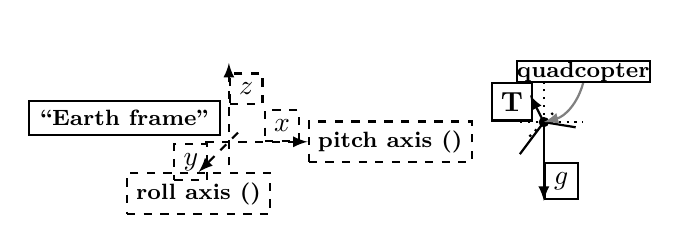
\begin{tikzpicture}

 \begin{scope}[yshift=-0.75cm]
 \draw[-latex,dashed] (-0.3,0,0) to node[near end,above] {$x$} (1,0,0) node[right] {\footnotesize pitch axis (\tlavar{\pitch})} ;
 \draw[-latex,dashed] (0,-0.3,0) to node[near end,right] {$z$} (0,1,0) ;
 \draw[-latex,dashed] (0,0,-0.3) to node[near end,left] {$y$} (0,0,1) node[below] {\footnotesize roll axis (\tlavar{\roll})} ;
 \node[anchor=east] at (-0.1,0.3,0) {\footnotesize ``Earth frame''} ;
 \end{scope}

 \rotateRPY{30}{-20}{0}

 \begin{scope}[xshift=4cm,yshift=-0.5cm]

   \draw[dotted] (-0.3,0,0) -- (0.5,0,0) ;
   \draw[dotted] (0,-0.3,0) -- (0,0.5,0) ;
   \draw[dotted] (0,0,-0.3) -- (0,0,0.5) ;

   \begin{scope}[RPY]
   \draw (0,0,0) to (0.5,0,0) ;
   \draw[-latex] (0,0,0) to node[near end,left] {\tlavar{T}} (0,0.5,0) ;
   \draw (0,0,0) to (0,0,0.5) ;
   \fill[black] (0,0,0) circle (0.05cm) ;
   \end{scope}

   \draw[latex-,gray] (0,0,0) to[bend right] (0.5,0.5) node[inner sep=0.1,anchor=south,black] {\footnotesize quadcopter} ; 

   \draw[-latex] (0,0,0) to node[near end,right] {$g$} (0,-1,0) ;
 \end{scope}

\end{tikzpicture}


\caption{Free-body diagram and dynamics of the quadcopter.}
\label{fig:free-body}
\end{figure}

Here \tlavar{T} represents the combined thrust of the motors (normalized
with respect to the mass of the quadcopter), \tlavar{\pitch} represents the
pitch (the angle around the $y$-axis), and \tlavar{\roll} represents the
roll (the angle around the $x$-axis). Figure~\ref{fig:free-body} depicts
this graphically in a free-body diagram. Our model is based on the
simplifying assumption (called the ``small angle condition'') that a
trusted attitude controller can instantaneously achieve any pitch and roll
within the bounds $-30\mydegree$ to $30\mydegree$ with a thrust greater
than or equal to 0, while holding yaw constant at 0.
\[
\smallangle \triangleq \left| \tlavar{\pitch} \right| \leq 30\mydegree \wedge \left|\tlavar{\roll}\right| \leq 30\mydegree \wedge 0 \leq \tlavar{T}
\]
Prior work has suggested that this is a reasonable approximation under this
small-angle condition ($\smallangle$), since the attitude dynamics are
significantly faster than the velocity and position
dynamics~\cite{Gillula2011}.  We capture this condition by requiring that
all quadcopter controllers are enabled under $\smallangle$.  That is, our
goal is to build controllers $D$ such that
\[
\begin{array}{l}
\SysPreservesP{I}{(\Sys{(D\wedge\Next{\smallangle})}{\W_{QC}}{\Delta})}~\wedge \\
\SysNeverStuckP{I}{(\Sys{(D\wedge\Next{\smallangle}))}{\W_{QC}}{\Delta})}
\end{array}
\]

For some state-constraints and their corresponding controllers, it is only
necessary to reason about an abstraction of the quadcopter dynamics
$\W_{QC}$.  For example, reasoning about a controller that enforces a bound
on the vertical position \tlavar{z} might only require reasoning about the
portion of the dynamics on which \tlavar{z} depends.  We formalize this
with:
\[\begin{array}{rl}
 & \SysPreservesP{I}{(\Sys{(D\wedge\Next{\smallangle}))}{\W}{\Delta})}~\wedge \\
 & \SysNeverStuckP{I}{(\Sys{(D\wedge\Next{\smallangle})}{\W}{\Delta})} \\
 & (\W_{QC} \rightarrow \W)~\wedge \\
\entails & \SysPreservesP{I}{(\Sys{(D\wedge\Next{\smallangle})}{\W_{QC}}{\Delta})}~\wedge \\
 & \SysNeverStuckP{I}{(\Sys{(D\wedge\Next{\smallangle})}{\W_{QC}}{\Delta})}
\end{array}
\]
where $\W_{QC} \rightarrow \W$ states that $\W$ is an abstraction of
$\W_{QC}$.

\subsection{Reuse via Substitution}
\label{sec:simulation}
\label{sec:subst}
Substitution of expressions for variables is a simple but powerful operator
that allows us to reuse controllers and their properties.  For example,
substitution allows us to perform familiar geometric transformations such
as translations, reflections, scaling, and rotations.  In addition,
substitution allows us to project simple dynamics onto more complex
dynamics; a technique we use to build verified state-constraining
controllers for the quadcopter.  We will explain the general technique by
using it to transport (re-use) the second-derivative controller
(\derivShimx), and its safety proof, to enforce a maximum altitude for our
quadcopter.

For a formula $P$ and substitution $\sigma$ (map from variables to
expressions), the semantic definition of substitution is:
\[\begin{array}{rcl}
tr \models \Rename{\sigma}{P} & \triangleq & \Rename{\sigma}{tr} \models P
\end{array}
\]
which states that a substituted formula ($\Rename{\sigma}{P}$) holds on a
trace ($tr$) if the formula ($P$) holds on the renamed trace
($\Rename{\sigma}{tr}$).  Under this definition, application of
substitution always guarantees preservation:
\begin{theorem}{\ProofRule{SubstPreserves}}
\begin{prooftree}
\AxiomC{$\entails \SysPreservesP{I}{S}$}
\UnaryInfC{$\entails \SysPreservesP{\big(\Rename{\sigma}{I}\big)}{\big(\Rename{\sigma}{S}\big)}$}
\end{prooftree}
\end{theorem}
This proof rule allows us to easily
transport \ProofRule{$\partial^2$-Preserves} to the quadcopter.  For
example, using it we can conclude
\begin{align*}
&\entails \SysPreservesP{\big(\Rename{\sigma_{\partial^2\rightarrow{}QC}}{\invShimx}\big)}{\big(\Rename{\sigma_{\partial^2\rightarrow{}QC}}{\derivShimx}\big)} \\
\sigma_{\partial^2\rightarrow{}QC} &\defined \{\tlavar{a} \mapsto \tlavar{T} \cos \tlavar{\roll} \cos \tlavar{\pitch} - g ,\; \tlavar{y} \mapsto \tlavar{z} ,\; \tlavar{v} \mapsto \tlavar{v_z}\}
\end{align*}
Note that the first argument to $\SysPreserves{}$ is the inductive
invariant for the new system, and can be read directly from the conclusion
of the preservation theorem.  This is the case for all of our preservation
theorems.

Next, we need to justify the \progress{} of the substituted system.  The
interaction between substitution and \progress{} is a bit subtle because
substitutions can introduce coupling between values that were uncoupled
before the substitution.  For example, $(\tlanextvar{x} =
1 \wedge \tlanextvar{y} = 0)$ is \Enabled{} while
$\Rename{\tlavar{x} \mapsto \tlavar{z}
,\; \tlavar{y} \mapsto \tlavar{z}}{(\tlanextvar{x} =
1 \wedge \tlanextvar{y} = 0)}$, which equals $\tlanextvar{z} =
1 \wedge \tlanextvar{z} = 0$, is not.

However, we can prove that \emph{invertible} substitutions preserve
progress.  This is because the inverse of the substitution is a function
for computing the \Enabledness witness for the substituted system from
the \Enabledness witness for the original system.  Because of this, we can
actually state a stronger \progress{} theorem for substitution, which
captures the fact that the inverse substitution preserves known constraints
on \Enabledness witnesses, such as $\Ca$ for the first and second
derivative controllers.  As we will see, this is crucial for proving the
small-angle constraint ($\smallangle$).  Formally,
\begin{theorem}{\ProofRule{Subst\xmakefirstuc{\progress{}}}}
For all formulas $S$, state formulas $Q$ and $R$, and substitutions
$\sigma$, if there exists a $\sigma^{-1}$ such that
$R\entails(\sigma \circ \sigma^{-1})\, \tlavar{x} = \tlavar{x}$ for all
variables \tlavar{x} that occur primed in $S$, and if
$R \entails \Rename{\sigma^{-1}}{Q}$ then
\begin{prooftree}
\AxiomC{$\entails \SysNeverStuckP{I}{(S\wedge\Next{R})}$}
\UnaryInfC{$\entails \SysNeverStuckP{\big(\Rename{\sigma}{I}\big)}{\big(\Rename{\sigma}{S}\wedge\Next{Q}\big)}$}
\end{prooftree}
\end{theorem}

When we apply this theorem to prove the \progress{} of the quadcopter
altitude controller, the following inverse works:
\[
\sigma_{\partial^2\rightarrow{}QC}^{-1} \triangleq \tlavar{\roll} \mapsto 0, \tlavar{\pitch} \mapsto 0, \tlavar{T} \mapsto \tlavar{a} + g, \tlavar{z} \mapsto \tlavar{y}, \tlavar{v_z} \mapsto \tlavar{v}
\]
We instantiate $Q$ with $\smallangle$ and $R$ with $\Ca$ to guarantee
\[
\SysNeverStuckP{I}{\big(\Sys{(\Rename{\sigma_{\partial^2\rightarrow{}QC}}{D_{\derivShimx}}\wedge \Next{\smallangle})}{(\Rename{\sigma_{\partial^2\rightarrow{}QC}}{\W_{1D}})}{\Delta}\big)}
\]

Finally, as noted above, we need to prove that
$\W_{QC} \rightarrow \Rename{\sigma_{\partial^2\rightarrow{}QC}}{\W_{1D}}$,
i.e. the continuous dynamics produced by the substitution is an abstraction
of the full quadcopter dynamics.  This reasoning involves standard
substation within differential equations, which we have formalized and
proved sound in Coq, and mechanical arithmetic reasoning.

\paragraph*{Enforcing Planar Boundaries}
Using our two substitution theorems, we can map the first- and
second-derivative controllers onto the quadcopter dynamics in many ways,
allowing us to verify many properties with relatively little effort.  We
showed how to use it to implement an upper bound on altitude.  In general,
we can use substitution on the second derivative controller to enforce that
the quadcopter stays on one side of any 2D plane in 3D space.  For example,
we can enforce a maximum-west boundary to prevent the quadcopter from
flying into a building.  Similarly, by applying substitution to the
first-derivative controller we can place bounds on velocity in any
direction.  The key is that our two substitution theorems allow us to
transfer the correctness of any controller to work on a new dynamics that
can be constructed from an invertible substitution.

\subsection{Disjunctive Composition}
\label{sec:disjunctive-composition}

In this section we present rules to compose systems using disjunction.  For
example, suppose that we wish to enforce a rectangular no-fly zone centered
around the origin (depicted in Figure~\ref{fig:dont-hit-the-pilot}).  A
system can avoid the no-fly zone if at all times it is to the north, the
south, the east, \emph{or} to the west of the rectangle.  We can build such
a system by disjoining subsystems $M_N$, $M_S$, $M_E$, and $M_W$, which are
each built from a substitution applied to \derivShimx{} to enforce the
northern, southern, eastern, and western boundaries of the box,
respectively.  As we will see, separately exposing preservation
and \progress{} allows us to define a disjunction operator that is fully
compositional and that permits the system to transition from an inductive
invariant of one subsystem to another (e.g. north of the no-fly zone to
west of the no-fly zone) during a single trace; this would not be possible
with global invariant proofs.

The disjunctive composition of two systems is defined by the $\oplus$
operator, which is indexed by the inductive invariants of the two systems.
Formally,
\begin{definition}{Disjunctive composition}
\[\begin{array}{l}
\SysDisjoin{\left(\Sys{D_1}{\W}{\Delta}\right)}{I_1}{\left(\Sys{D_2}{\W}{\Delta}\right)}{I_2} \triangleq \\
\qquad \Sys{\big((I_1 \wedge D_1) \vee (I_2 \wedge D_2)\big)}{\W}{\Delta} %% \big((I_1 \wedge \W_1) \vee (I_2 \vee \W_2)\big)}{\Delta}
\end{array}
\]
\end{definition}
The inclusion of the \emph{inductive} invariants in this definition is
essential to enforce the disjunction of the properties.  To see why,
consider our example and suppose the system is currently along the western
edge of the no-fly zone.  Since the system is outside of the inductive
invariant of the eastern controller, the eastern controller could allow the
system to do anything, including moving east into the no-fly zone.  Thus,
at each discrete transition, the composed controller must consider the
discrete transitions of a sub-controller whose inductive invariant
currently holds.  This guarantees that the inductive invariant of that
subsystem holds after the transition.  Moreover, it means that the system
can transition from one inductive invariant to another, only where the
inductive invariants overlap.

\begin{figure}[t]
\centering
\begin{tikzpicture}[x=1cm,y=1cm]

\begin{scope}[yscale=0.75,xscale=0.75]

% Axis
\draw (-3,0) -- (3,0) ;
\draw (0,-3) -- (0,3) ;


\draw[dashed] (-1.75,-3) -- (-1.75,3) ;
\fill[pattern=north west lines, pattern color=gray] (-1.75,-3) rectangle (-3,3) ;

\begin{scope}[rotate=180]
\draw[dashed] (-1.75,-3) -- (-1.75,3) ;
\fill[pattern=north west lines, pattern color=gray] (-1.75,-3) rectangle (-3,3) ;
\end{scope}

\begin{scope}[rotate=90]
\draw[dashed] (-1.5,-3) -- (-1.5,3) ;
\fill[pattern=north east lines, pattern color=gray] (-1.5,-3) rectangle (-3,3) ;
\end{scope}

\begin{scope}[rotate=-90]
\draw[dashed] (-1.5,-3) -- (-1.5,3) ;
\fill[pattern=north east lines, pattern color=gray] (-1.5,-3) rectangle (-3,3) ;
\end{scope}

\node[anchor=west,fill=white,opacity=0.75,inner sep=0.15em] at (-2.7,2.5) {\small Safe Region} ;
\node[anchor=west,inner sep=0.15em] at (-2.7,2.5) {\small Safe Region} ;

\node[anchor=west,fill=white,opacity=0.75,inner sep=0em,text width=1.25cm,align=center] at (-1.75,0.5) {} ;
\node[anchor=west,inner sep=0em,text width=2cm,align=center] at (-1.5,0.1) {\small Restricted Zone} ;

\draw[latex-] (2,2) to[bend left] (3.5,2) node[inner sep=0.15em,anchor=north west,text width=3.5cm] {\footnotesize Intersection of inductive invariants} ;

\draw[latex-] (-2,0.1) to[bend right] (-3.5,0.4) node[inner sep=0.15em,anchor=east] {\footnotesize $M_W$} ;
\draw[latex-] (-1,1.75) to[bend left] (-3.5,2.1) node[inner sep=0.15em,anchor=south east] {\footnotesize $M_N$} ;
\draw[latex-] (-1,-1.75) to[bend left] (-3.5,-2.1) node[inner sep=0.15em,anchor=south east] {\footnotesize $M_S$} ;

\draw[latex-] (2,-0.5) to[bend right] (3.5,-1.2) node[inner sep=0.15em,anchor=west] {\footnotesize $M_E$} ;

\end{scope}
\end{tikzpicture}


\caption{Staying out of restricted airspace using the disjunction of four controllers.}
\label{fig:dont-hit-the-pilot}
\end{figure}

This definition of disjunction is fully compositional with
both \SysPreserves and \SysNeverStuck.  In particular, the disjunctive
composition of two systems that independently preserve $I_A$ and $I_B$
preserves $I_A \vee I_B$:
\begin{theorem}{\ProofRule{DisjoinPreserves}}
\[\begin{array}{rl}
       & \SysPreservesP{I_A}{A} \;\wedge\; \SysPreservesP{I_B}{B} \\
\entails & \SysPreservesP{\big(I_A \vee I_B\big)}{\big(\SysDisjoin{A}{I_A}{B}{I_B}\big)}
\end{array}
\]
\end{theorem}
\noindent
Using only this theorem we can easily construct a proof that the
disjunctive composition of our four controllers enforces the no-fly zone
property.

A similar theorem states that \disjoinop guarantees \SysNeverStuck.
\begin{theorem}{\ProofRule{Disjoin\xmakefirstuc{\progress{}}}}
\[\begin{array}{rl}
       & \SysNeverStuckP{I_A}{A} \;\wedge\; \SysNeverStuckP{I_B}{B} \\
\entails & \SysNeverStuckP{(I_A \vee I_B)}{\big(\SysDisjoin{A}{I_A}{B}{I_B}\big)}
\end{array}
\]
\label{thm:progress-disjoint}
\end{theorem}
\noindent
The proof follows from the fact that $I_A$ ensures the \Enabledness of $A$
and $I_B$ ensures the \Enabledness of $B$.  Since the new inductive
invariant $\left( I_A \vee I_B\right)$ ensures that at least one of $I_A$
or $I_B$ holds, at least one of $A$ or $B$ must be \Enabled.

Disjunction is a very powerful composition mechanism that is applicable in
a wide variety of circumstances.  For example, we can use it to guarantee
that a train can only have a high velocity when it is not in a curve by
composing a maximum velocity controller with a controller that stops the
train before curves.  A controller such as this one could have prevented
the Amtrak derailment in Philadelphia in 2015 that killed 8 people and
injured 200.

\subsection{Conjunctive Composition}
\label{sec:conjunctive-composition}

In this section, we present rules to compose systems to ensure the
conjunction of their properties.  For example, one might want to ensure
that a system's upward velocity does not exceed 1 m/s \emph{and} that the
system stays below 100m by conjoining the first and second derivative
controllers.  Unlike disjunctive composition, conjunctive composition of
two systems satisfying \progress{} does not guarantee a system
satisfying \progress{}, due to coupling.  However, our ability to
separately prove \progress{} allows us to push forward.  We show that, even
in coupled domains, conjunctive composition can lead to substantial savings
in proof effort, and demonstrate some clever tricks that allow us to
decouple domains that, on the surface, seem intricately linked.

We use the same definition for conjoining systems as in Chapter~\ref{chap:memo15}.
We restate the definition here for clarity:
\sysconjoin*
The crucial feature of this definition is how it interacts
with \SysPreserves.  Note that while disjunctive composition requires that
both systems have the same continuous transition, conjunctive composition
does not impose this restriction.
\begin{theorem}{\ProofRule{ConjoinPreserves}}
\[\begin{array}{rl}
       & (I_B \rightarrow \SysPreservesP{I_A}{A}) \;\wedge\; (I_A \rightarrow \SysPreservesP{I_B}{B}) \\
\entails & \SysPreservesP{\big(I_A \wedge I_B\big)}{\big(\SysConjoinP{A}{B}\big)}
\end{array}
\]
\label{thm:conjoin-preserves}
\end{theorem}
Intuitively, if we start in a state satisfying both $I_A$ and $I_B$, $A$
guarantees that we stay in $I_A$, and $B$ guarantees that we remain in
$I_B$, then if both $A$ and $B$ hold, we must remain in the intersection of
$I_A$ and $I_B$. Note that Theorem~\ref{thm:conjoin-preserves} removes the
restriction of acyclic parallel composition from
Theorem~\ref{thm:sys-compose} in Chapter~\ref{chap:memo15}. This is
possible because the inductive invariants are made explicit.

The difficulty of conjunctive composition lies in justifying \progress{}.
Even though $A$ and $B$ may independently be \Enabled under the inductive
invariant, there is no guarantee that their conjunction is \Enabled.  For
example, suppose that we wish to compose an overly-conservative upper-bound
controller that insists on a negative acceleration and a similarly
conservative lower-bound controller that insists on a positive
acceleration.  Since acceleration can not be simultaneously positive and
negative, the conjunction of these controllers does not
satisfy \progress{}.

Nevertheless, all is not lost when conjoining two systems.  There are a
variety of techniques for proving \Enabledness of conjunctions.  We will
illustrate these techniques through a sequence of examples, ultimately
culminating in a 3D bounding box for both position and velocity.

\paragraph*{Example: Staying within an Interval}
Consider constructing a controller that enforces both an upper and a lower
bound on both position ($y$) and velocity ($v$) in a single spatial
dimension.  We can build such a controller (which we call \intervalShim)
using $\SysConjoin$ and an application of our substitution operator to the
second- and first-derivative controllers:
\begin{align*}
\intervalShim &\defined \SysConjoinP{\derivShimx}{\Rename{\mirrorx}{\derivShimx}} \SysConjoin \derivShimv \SysConjoin \Rename{\mirrorx}{\derivShimv} \\
\mirrorx &\defined \{ \tlavar{y} \mapsto -\tlavar{y} ,\; \tlavar{v} \mapsto -\tlavar{v} ,\; \tlavar{a} \mapsto -\tlavar{a} \}
\end{align*}
Here, the $\mirrorx$ substitution mirrors the controller's logic so that
rather than enforcing an upper bound on $\tlavar{y}$ of $\ubY$ (resp. $v_y$
of $v_{\mathsf{ub}}$), the substituted controller enforces a lower bound on
$\tlavar{y}$ of $-\ubY$ (resp. $v_y$ of $-v_{\mathsf{ub}}$).

The preservation of this composition follows immediately
from \ProofRule{ConjoinPreserves}, \ProofRule{$\partial^2$-Preserves}, \ProofRule{$\partial$-Preserves},
and \ProofRule{SubstPreserves}.  However, since conjoined systems are not
guaranteed to satisfy \progress{}, we must prove this separately.
Formally, we must prove \progress{} of $\intervalShim$ under the
conjunction of the inductive invariants of the subsystems:
\footnote{For brevity, $\invShimx$ and $\invShimv$ refer to the inductive invariants of \derivShimx{} and \derivShimv{}.}
\[
\SysNeverStuckP{\big(\invShimx\wedge\Rename{\mirrorx}{\invShimx}\wedge\invShimv\wedge\Rename{\mirrorx}{\invShimv}\big)}{\intervalShim}
\]

Informally, this states that, under the inductive invariant, there exists
an action that is acceptable to all of the (non-deterministic) controllers.
More formally, we must justify that there does not exist any state
satisfying the inductive invariant for which there is not an action that
all controllers accept.  Unfolding the definitions and applying the
substitution ($\mirrorx$) reveals that the \progress{} of $\intervalShim$
reduces to first-order reasoning over real arithmetic.  At first glance, it
may seem as though modularity was a failure here; however, by separating
preservation and \progress{}, the non-modularity of \progress{} did not
prevent us from modularly proving preservation.  Moreover, our split
crucially allows us to assume the inductive invariant when
proving \progress{}.

This is in contrast to other work~\cite{alur1997modularity} where
conjunctive (parallel) composition is only allowed when the individual
modules output to disjoint sets of variables.  Furthermore, we found the
proof of $\SysNeverStuckP{I_{\intervalShim}}{\intervalShim}$ to
be \emph{less than one third} the size of the proof of preservation of the
individual second-derivative controller \derivShimx.  This means that
$\SysConjoin$ greatly reduces the cost of conjoining systems, even when
these systems are tightly coupled.

It is important to note that under-specification of controllers is
essential to composition in this case.  If both systems were completely
specified then the two systems would be forced to make identical choices in
order for them to compose.  By composing under-specified controllers, we
retain the flexibility to find a solution that reconciles the restrictions
of both controllers.

In certain cases, our proof rules can be used to verify \progress{}
compositionally.  To demonstrate this, we turn to the task of using our
interval controller to modularly build a bounding rectangular prism.  We
approach the problem in three steps.  First, we compose two interval
controllers to enforce a bounding box in two spatial dimensions.  In the
next section, we adapt this controller to the quadcopter by incorporating
the small-angle constraint.  Finally, we apply the same technique to extend
the 2D box into a 3D prism.

\paragraph*{Example: Conjunction of Independent Systems}
We construct the box by conjoining two instances of $\intervalShim$, using
substitution to map them to the $x$- and $z$-dimensions respectively.
\[\begin{array}{rcl}
\mathsf{Box} & \defined & \Rename{\sigma_x}{\intervalShim} \SysConjoin \Rename{\sigma_z}{\intervalShim} \\
\sigma_x &\defined &\{ \tlavar{y} \mapsto \tlavar{x} ,\; \tlavar{v} \mapsto \tlavar{v_x} ,\; \tlavar{a} \mapsto \tlavar{a_x} \} \\
\sigma_z &\defined & \{ \tlavar{y} \mapsto \tlavar{z} ,\; \tlavar{v} \mapsto \tlavar{v_z} ,\; \tlavar{a} \mapsto \tlavar{a_z} - g \}
\end{array}
\]
Verifying that $\mathsf{Box}$ enforces a bounding box is simply a matter of
using \ProofRule{ConjoinPreserves}, \ProofRule{SubstPreserves}, and the
preservation proof of $\intervalShim$.

As others have noted~\cite{alur1997modularity}, \progress{} of conjoined
systems is compositional, if the two systems output to disjoint sets of
variables.  In our logic, the output variables of a formula are the
next-state (primed) variables, whose disjointness is expressed by $A \perp'
B$.  Formally,
\begin{theorem}{\ProofRule{Conjoin\xmakefirstuc{\progress{}}Disjoint}}
For all systems $A$ and $B$ such that $A \perp' B$, and for all state formulas $I_A$ and $I_B$,
\[\begin{array}{rl}
       & \SysNeverStuckP{I_A}{A} \;\wedge\; \SysNeverStuckP{I_B}{B} \\
\entails & \SysNeverStuckP{\big(I_A \wedge I_B\big)}{\big(\SysConjoinP{A}{B}\big)}
\end{array}
\]
\end{theorem}
While we can not express disjointness of primed variables ($A \perp' B$)
formally within our temporal logic, we can capture it in Coq's logic.
Further, in practice the disjointness of two formulas is easily decidable
in many cases meaning that discharging this side condition is often
trivial.  From this theorem and variable disjointness, $\mathsf{Box}$
satisfies \progress{} for the dynamics with independent \tlavar{a_x}
and \tlavar{a_y}.

Now suppose that instead of rectangular dynamics with independent control
inputs \tlavar{a_x} and \tlavar{a_y}, we want a controller for polar
coordinates with independent control inputs \tlavar{a} and \tlavar{\pitch}.
For example, these are the dynamics of a 2D version of the quadcopter (with
$\tlavar{\roll}$ fixed at 0), in the absence of the small-angle constraint.
While the transformation to polar coordinates seems to couple the $x$ and
$z$ instantiations of $\intervalShim$, there is always an invertible map
from rectangular to polar coordinates.  This connection between polar and
rectangular coordinates allows us to use the substitution theorems from
Section~\ref{sec:subst} to prove both preservation and \progress{} for a
version of $\mathsf{Box}$ that operates using polar thrust.

Note that to arrive at this result, we first used disjoint composition to
justify the syntactically independent system satisfies \progress{}.  We
then applied our substitution theorems and the invertibility of the
rectangular-to-polar transformation to show that the resulting system was
the same as the quadcopter dynamics modulo the small-angle constraint. The
takeaway is that although the system
($\Rename{\sigma_{\pitch}}{\mathsf{Box}}$) is not superficially composed of
disjoint subsystems, we can still verify both \progress{} and preservation
fully modularly.

\paragraph*{Example: Incorporating the Small-angle Constraint}
The previous example ignored the small-angle constraint, which is critical
to the accuracy of our model of the quadcopter's dynamics.  In this section
we address this shortcoming and complete the verification of $\mathsf{Box}$
with respect to a 2D version of $\W_{QC}$ (again, with $\tlavar{\roll}$
fixed at 0) \emph{in a fully modular way}.  Figure~\ref{fig:small-angle}
shows how the small-angle constraint introduces coupling into the
independent box.  In particular, the hatched region corresponds to the
accelerations achievable under the small-angle constraint while the
unconstrained region corresponds to the accelerations necessary for
$\mathsf{Box}$ developed in the previous section.

\newcommand{\Tminx}{\ensuremath{\Tmin^{x}}\xspace}
\newcommand{\Tminz}{\ensuremath{\Tmin^{z}}\xspace}

\begin{figure}[t]
\centering
\begin{tikzpicture}[x=0.48cm,y=0.48cm]

\draw[latex-latex] (0,-2) -- (0,2) node[above] {$z$};
\draw[latex-latex] (-2,0) -- (2,0) node[anchor=west] {$x$};

\draw[-latex] (0,-1.5) -- (45:3) ;
\draw[-latex] (0,-1.5) -- (135:3) ;
\fill[pattern color=gray!50,pattern=north west lines] (0,-1.5) -- (45:3) -- ++(-4.25,0) -- cycle ;

\draw[densely dotted,thick] (-1.5,-1.5) rectangle (1.5,1.5) ;

\draw[dashed] (-0.6,-0.5) rectangle (0.6,0.5) ;

\begin{scope}[xscale=-1]

\draw[latex-,gray] (1.7,1.75) to[bend left] (3,1) node[anchor=north east,inner sep=0.2,black] {\footnotesize small-angle achievable} ;
\draw[latex-,gray] (1,-1) to[bend left] (3,-1) node[anchor=north east, inner sep=0.2,black] {\footnotesize unconstrained \Tminx, \Tminz} ;
\draw[latex-,gray] (-0.2,0.2) to[bend right] (-3,1.0) node[anchor=west,inner sep=0.2,black,text width=3.5cm] {\footnotesize independently achievable} ;

\end{scope}
\end{tikzpicture}

\caption{Decoupling of \tlavar{a_x} and \tlavar{a_z}.}
%%\caption{\tlavar{a_x} and \tlavar{a_z} can be decoupled under the small-angle constraint under assumptions on their ranges.}
\label{fig:small-angle}
\end{figure}

Our approach relies on a detail of the verification which we glossed over
in the previous presentation.  In particular, because the second-derivative
controller is \emph{parameterized by \Tmin}, $\mathsf{Int}$ is
parameterized by an \Tmin and $\mathsf{Box}$ is parameterized by a pair
of \Tmin's in the $x$ and $z$ dimensions.  The right side of
Figure~\ref{fig:small-angle} shows how we leverage the parameterization of
$\mathsf{Box}$ to logically decouple the two dependent dimensions.  Our
insight is the following.  If we can pick values for \Tminx and \Tminz
(note that \Tminx and \Tminz are negative) such that all accelerations
$a_x$ and $a_z$ where $|a_x| \leq -\Tminx$ and $|a_z| \leq -\Tminz$ are
achievable by \tlavar{T} and \tlavar{\pitch} under the small-angle
constraint then the values of \tlavar{a_x} and \tlavar{a_z} can be chosen
independently \emph{if they fall within the bounds}.  Purely trigonometric
reasoning reveals that the constraint on \tlavar{\pitch} is achieved for
any values of \tlavar{a_x} and \tlavar{a_z} satisfying
$\xConstraint \wedge \zConstraint$ defined as:
\begin{align*}
\xConstraint &\defined -(\Tmin + g) \tan 30\mydegree \leq \tlavar{a_x} \leq  (\Tmin + g) \tan 30\mydegree \\
\zConstraint &\defined \Tmin \leq  \tlavar{a_z}  \leq   -\Tmin
\end{align*}

We can formalize this reasoning by noting that the previous example
($\mathsf{Box}$), instantiated with the above choices of $\Tminx$ and
$\Tminz$, satisfies \progress{} under the constraint
$\xConstraint \wedge \zConstraint$.  Thus, we can use the substitution
proof rule \ProofRule{Subst\xmakefirstuc{\progress{}}} with a
rectangular-to-polar substitution, instantiating $R$ with
$(\xConstraint\wedge\zConstraint)$ and $Q$ with the small-angle condition
(ignoring $\tlavar{\roll}$ since it is assumed to be 0 in this 2D example).

The important point of this verification is that the separation of
preservation and \progress{} allowed for a relatively small and modular
proof of a complex property of a \emph{highly coupled system}.  Without the
separation of preservation and \progress{}, the coupling would have forced
us to re-prove many of the intermediate properties.

\paragraph{Example: Adding the Third Dimension}
We can build a controller enforcing a cube by conjoining $\mathsf{Box}$
with another instance of $\intervalShim$ substituted to reflect the $y$
dimension.  We can then apply this cube to the 3D version of $\W_{QC}$
(including $\tlavar{\roll}$ and the coupling small-angle constraint).
Again, the modularity of our proofs shields us from much of the complexity.
$\mathsf{Box}$ enforced the constraints for \tlavar{x} and \tlavar{z}
using \tlavar{a_x} and \tlavar{a_z}.  Extending this to handle the third
dimension simply requires that we use substitution to view \tlavar{a_x}
and \tlavar{a_z} as a single unit and carry out the same reasoning,
independently controlling that composed unit and \tlavar{a_y}.

\section{Evaluation}
\label{sec:eval}
We evaluate our approach with four criteria: (1) proof effort, (2)
expressiveness, (3) flight behavior, and (4) comparison to fully automated
tools.

\subsection{Proof Effort}
Table~\ref{fig:monitors} lists all of the geofencing controllers that we
verified and flew, along with the composition mechanism, proof size, and
number of symbols in the discrete transition for each one.  The first 2
rows list controllers that we ported from prior work; these are our atomic
building blocks.  The next 3 rows list controllers that we built and
verified using a combination of substitution and conjunction.  The
remaining rows list controllers that we built using disjunction and
substitution.

\begin{table}
\caption{Systems implemented and proved correct. The first column is the name of the system. The second column shows how each system was built and proved correct from smaller components. $\Rename{}{i}$ indicates a substitution applied to system $i$ (we have omitted the specific substitution); $\SysConjoin$ represents conjunction composition; and $\disjoinop$ represents disjunction composition. The third and fourth columns show the number of symbols in the discrete controller and the number of lines of proofs, respectively.}
\label{fig:monitors}
\begin{tabular}{l|l|r|r}
id: Name & Built How? & \# of Symbols & Lines of Proof \\
\hline 
a: 1D velocity bound & From Scratch & 43 & 130 \\
b: 1D position bound & From Scratch & 126 & 484 \\
c: 1D interval & $\SysConjoinP{\SysConjoinP{\Rename{}{b}}{\Rename{}{b}}}{\SysConjoinP{\Rename{}{a}}{\Rename{}{a}}}$ & 323 & 194 \\
d: 2D square & $\Rename{}{(\SysConjoinP{\Rename{}{c}}{\Rename{}{c}})}$ & 805 & 258 \\
e: 3D cube & $\Rename{}{(\SysConjoinP{d}{\Rename{}{c}})}$ & 1353 & 201 \\
f: 3D square donut & $\Rename{}{e}\disjoinop\Rename{}{e}\disjoinop\Rename{}{e}\disjoinop\Rename{}{e}$ & 5412 & 23 \\
g: 3D +, T, $\bot$ & $\Rename{}{e}\disjoinop\Rename{}{e}\disjoinop\Rename{}{e}\disjoinop\Rename{}{e}$ & 5412 & 23 \\
h: 3D pilot box & $\Rename{}{e}\disjoinop\Rename{}{e}\disjoinop\Rename{}{e}\disjoinop\Rename{}{e}$ & 5412 & 23 \\
\end{tabular}
\end{table}

Note that our 1D position controller ($b$ in Table~\ref{fig:monitors})
involves 3 variables and 126 symbols and is a relatively simple discrete
transition requiring only multiplication and addition.  However, verifying
this position controller required substantial, tedious, manual proof effort
because of the difficulty of reasoning about nonlinear real arithmetic.  On
the other hand, our 3D cube controller ($e$ in Table~\ref{fig:monitors})
contains 9 variables, 1353 symbols, trigonometric functions, and angular
constraints.  This increase in complexity is actually quite daunting for
two reasons: (1) arithmetic decision procedures have very bad worst case
complexity, and (2) trigonometric functions make the problem
undecidable~\cite{HarrisonLogic09}.  Despite the substantial increase in
complexity, our modular verification approach allowed us to verify the 3D
version with only a modest amount of additional manual proof effort.

Moreover, note that all controllers built using disjunction require
negligible proof effort on top of the effort required to verify the
individual components.  This is because disjunction composes proofs of both
preservation and \progress{}. As we discuss in the next subsection, this is
a very powerful tool.

Finally, it is worth noting that we have several admits in our Coq
development: (1) basic arithmetic theorems, (2) some theorems bridging the
gap between $\W_{QC}$ and its abstractions, (3) theorems
stating \progress{} of the continuous transitions in the quadcopter model.
Crucially, these admits do not interfere with the core ideas that we are
exploring, namely modular reasoning about sampled-data systems.

\subsection{Expressiveness}
Disjunction is extremely powerful when building real-world controllers.
For example, we can build up pixelated versions of arbitrary shapes by
composing instances of our cube controller.  Interesting properties that we
can build with this include: (1) avoid no-fly zones such as airports, the
white house, etc, (2) do not fly within a box surrounding the pilot, (3)
stay away from static barriers such as trees and buildings, and (4) avoid
skyscrapers in a city. In fact, our disjunction rules can be used to
compose \emph{any} controller with any other controller, not just a cube.
For example, if we were able to verify a controller enforcing a triangular
prism or a sphere, we could compose instantiations of these controllers
with our existing cube, with each other, or with any other controller.
Again, all of this requires negligible additional proof burden.

Conjunctive composition is similarly expressive -- the box and the cube
both make heavy use of conjunctive composition.  The proof burden when
using conjunction comes from justifying \progress{} (progress) of the
resulting systems, which is not as compositional, especially in highly
coupled domains.  Nevertheless, Our separation of \progress{} (progress)
and preservation makes it possible to build compositional proofs of
preservation even in highly coupled domains such as the box and cube.
Finally, substitution allows us to reuse all controllers by translating and
rotating them, and by transforming them into controllers for different
physical dynamics.

\subsection{Behavior in Actual Flight}
\label{sec:flight}
To make sure that our controllers work well in practice, we manually
translated our models to C and ran them on a 3DR Iris+ quadcopter.  This
allows us to evaluate the accuracy of our approximations.
Figure~\ref{fig:emsoft-arch} depicts the architecture of the system with one of
our controllers inserted.  Our controllers check the outputs of the
pre-existing control software, potentially replacing them with default safe
values; this resolves the non-determinism of the controller specifications.
This architecture means that the behavior of much of the existing control
software (left of ``Verified Control'') cannot cause a violation of the
fence.  Moreover, if the quadcopter remains sufficiently far from the fence
boundaries, the system behaves exactly as it would without our controllers,
so any performance properties of the existing control software are
preserved.

\begin{figure}[t]
  \centering
  \begin{tikzpicture}
    \tikzstyle{every node}=[draw=black,thick,font=\bfseries,node distance=0.35cm]
    \tikzstyle{every path}=[draw=black,thick]
    \tikzstyle{wnode}=[minimum height=1cm]

    \node[fill=black,text=white,text width=2cm,align=center,minimum height=1cm] (mon) at (0,0) {Verified Control} ;
    \node[wnode,left=of mon,text width=2cm,align=center] (existing)  {Existing Control Software} ;

    \node[draw=black,left=of existing,minimum height=0.5cm,yshift=0.3cm] (user) {User} ;
    \node[draw=black,left=of existing,minimum height=0.6cm,yshift=-0.8cm] (sensor) {Sensors} ;

    \node[wnode,right=of mon,text width=2cm,align=center] (control)  {Attitude Control} ;
    \node[wnode,right=of control] (motor)  {Motors} ;

    \newcommand{\quadline}[2]{%
    \foreach \i in {-2,...,1}{%
      \draw[-latex] ([yshift=0.12cm + \i * 0.24 cm]#1.east) -- ([yshift=0.12cm + \i * 0.24 cm]#2.west) ;}}

    \quadline{mon}{control}
    \quadline{control}{motor}
    \quadline{existing}{mon}
    \draw[-latex] let \p1 = (user.east),
                      \p2 = (existing.west) in
                  (user.east) -- (\x2,\y1) ;
    \draw[-latex] let \p1 = (sensor.east),
                      \p2 = (existing.west) in
                  ([yshift=0.2cm]sensor.east) -- (\x2,\y1+0.2cm) ;
    \draw[-latex] ([yshift=-0.2cm]sensor.east) -| (mon.south) ;



  \end{tikzpicture}

     \caption{System architecture.}
     \label{fig:emsoft-arch}
\end{figure}

We flew our quadcopter with all controllers listed in
Table~\ref{fig:monitors}.  All of the controllers enforced their
respective bounds with only minor violations, which can be attributed to
un-modeled forces such as wind and to modeling approximations.

Perhaps the largest gap between our temporal logic model and the real world
comes from our assumption that the controllers can instantaneously set the
orientation, or attitude, of the quadcopter
(Section~\ref{sec:quadcopter-dynamics}).  This is not possible in reality.
Instead, an attitude controller controls attitude indirectly by sending
voltage signals to the quadcopter's motors.  Thus, our controllers output
desired attitude values (i.e. roll and pitch) to an attitude controller,
and assume that these values are achieved instantaneously.  Prior work has
suggested that this is a reasonable approximation, under the small angle
assumption, since the attitude dynamics are significantly faster than the
velocity and position dynamics~\cite{Gillula2011}.  Nevertheless, one of
the reasons for running our controllers on a real quadcopter is to
experimentally evaluate whether the attitude assumption works well in our
context.

Manually translating our models to C introduces a potential source of
errors.  The two main aspects of this translation are: (1) approximating
infinite precision real numbers in the logic using floating point numbers,
and (2) validating the assumptions about the runtime of code using
worst-case execution time analysis on the resulting code.  Both of these
problems have been explored in a variety of
contexts~\cite{darulova2014sound,maroneze2014certified,wilhelm2008worst},
and are orthogonal to modularity.

Our experiences flying the controllers from this chapter suggest several
interesting avenues for future study.  First, our controllers can cause the
quadcopter to oscillate near the boundaries.  If the pilot commands maximum
acceleration towards a boundary, then our controllers, rather than
converging smoothly to zero acceleration at the boundary, ultimately
oscillate quickly between the pilots desired acceleration and the
controller's breaking acceleration.  This is due to a large discontinuity
in control input (desired attitude) near the boundaries. We address this
shortcoming in Chapter~\ref{chap:exp-smpl}.

Second, an early C implementation of our multi-cube controller (formed from
a disjunction of cubes), was overly conservative due to the logic it used
for responding to violations of both controllers.  In particular, it
sometimes prevented the quadcopter from leaving a particular cube, even
though the desired quadcopter path was safe for another cube.  The solution
was to break ties in favor of the least invasive choice, which is a
heuristic not expressed in the model. This experience suggests the some
sort of liveness property is an interesting avenue for future work in this
domain.
 
Finally, our results suggest that minor violations of even formally
verified properties are inevitable since no useful model of the physical
world can capture everything.  Most of the time our controllers work well
outside the boundaries, but our experiments do show that occasionally they
cause the quadcopter to temporarily get stuck outside the boundaries. This
means that it would be valuable to prove stronger versions of our state
invariants expressing a form of robustness. Here, we can build on
robustness notions from control theory called input-to-state
stability~\cite{ISSsontag2008} and input-to-state dynamical
stability~\cite{gruneISDS02}.  These definitions state that the behavior of
a system \emph{degrades gracefully} as disturbances grow and that the
effect of individual disturbances decreases as time passes.  For example, a
quadcopter running our controllers may violate the boundary by a small
amount if there is a small amount of wind and by a large amount if there is
a strong wind, but in the absence of wind the vehicle must re-enter the
boundary.

\subsection{Comparison with fully automated tools}
There are a number of state-of-the-art tools that attempt to automatically
verify hybrid
systems~\cite{PHAVerSTTT08,chen2015flow,kong2015dreach,HyTechCAV97}, but
due to the complexity of the domain, they are limited to certain classes of
systems and properties.

PHAVer~\cite{PHAVerSTTT08}, which we ran through the SpaceEx tool
platform~\cite{frehse2011spaceex-small}, is able to verify only one of our
systems, namely the combined upper and lower bound on velocity.  However,
PHAVer is not able to verify the upper bound on velocity in isolation,
probably because there are fewer constraints on acceleration to limit the
search space, compared to the controller that bounds velocity from above
and below.  Finally, PHAVer is not able to run any of our other systems
because the discrete transitions involve non-linear arithmetic; analyzing
these systems would require manual construction of a linear
overapproximation of the discrete transitions.

dReach~\cite{kong2015dreach} and Flow*~\cite{chen2015flow}
are \emph{bounded} model checkers, which means that they can conclude
safety of a system within a user-specified time bound.  Our Coq proofs, on
the other hand, guarantee safety for infinite runs.  It is possible to use
dReach and Flow* to guarantee safety for all runs by manually providing the
inductive invariant.  In this way, our results are complementary, as they
provide a decomposition technique to manage scalability issues of these
tools.  However, these tools are currently unable to handle universally
quantified variables with unbounded domains.  This prevents them from
verifying safety of systems with symbolic parameters, such as $\amin$ --
they require concrete numerical bounds on these parameters, which weakens
the safety theorem.

\section{Acknowledgments}
This chapter, \emsoftack{}
